\documentclass{article}
\usepackage{amsmath,amssymb,graphicx,algpseudocode,algorithm,amsthm}
\usepackage[margin=1in]{geometry}
\usepackage{mathrsfs}
\let\mathcrl\mathscr
\usepackage[mathscr]{euscript}
\usepackage{marginnote}
\usepackage{hyperref}
\usepackage{qtree}
\usepackage{graphicx}
\usepackage{tikz}
\geometry{reversemarginpar}

\author{Benji Altman}

\def\latex{\LaTeX\ }

\newcommand{\comment}[1]{}
\def\useLim{\limits}
\newcommand{\question}[1]{\marginnote{#1}}
\let\union\cup
\let\inter\cap
\let\emptyset\varnothing
\let\bigunion\bigcup
\let\biginter\bigcap
\let\composed\circ
\let\cross\times
\def\And{\textit{ and }}
\def\Or{\textit{ or }}
\def\sbSeperator{\,\middle|\,}
\def\Return{\State\textbf{return}\par}
\def\ZNonNegative{{\mathbb Z_{\ge 0}}}
\newcommand{\setcomp}[1]{{#1}^{\mathsf{c}}}
\newcommand{\prodfrom}[3]{\prod\useLim_{#1}^{#2}\LB {#3} \RB}
\newcommand{\sumfrom}[3]{\sum\useLim_{#1}^{#2} \LB {#3} \RB}
\newcommand{\unionfrom}[3]{\bigunion\useLim_{#1}^{#2} \LB {#3} \RB}
\newcommand{\interfrom}[3]{\biginter\useLim_{#1}^{#2} \LB {#3} \RB}
\newcommand{\interacross}[2]{\interfrom{#1}{}{#2}}
\newcommand{\unionacross}[2]{\unionfrom{#1}{}{#2}}
\newcommand{\sumacross}[2]{\sumfrom{#1}{}{#2}}
\newcommand{\prodacross}[2]{\prodfrom{#1}{}{#2}}
\newcommand{\Lim}[3]{\lim\useLim_{{#1} \to {#2}}\LB {#3} \RB}
\newcommand{\set}[1]{\left\{ {#1} \right\}}
\newcommand{\setbuilder}[2]{\left\{{#1} \sbSeperator {#2}\right\}}
\newcommand{\derivative}[2]{\frac{d}{d{#2}}\LB {#1} \RB}
\newcommand{\Exists}[2]{\exists_{#1}\LB {#2} \RB}
\newcommand{\All}[2]{\forall_{#1}\LB {#2} \RB}
\newcommand{\abs}[1]{\left|{#1}\right|}
\newcommand{\card}[1]{\left| {#1} \right|}
\newcommand{\range}[1]{\textit{\textbf{Rng}}\left( {#1} \right)}
\newcommand{\domain}[1]{\textit{\textbf{Dom}}\left( {#1} \right)}
\newcommand{\pset}[1]{\mathcal P\left( {#1} \right)}
\newcommand{\pair}[2]{\left( {#1} , {#2} \right)}
\def\closure{\overline}
\newcommand{\limpts}[1]{{#1} '}
\newcommand{\ooint}[2]{\left( {#1} , {#2} \right)}
\newcommand{\ocint}[2]{\left( {#1} , {#2} \right]}
\newcommand{\coint}[2]{\left[ {#1} , {#2} \right)}
\newcommand{\ccint}[2]{\left[ {#1} , {#2} \right]}
\newcommand{\eqclass}[1]{\bar{#1}}
\newcommand{\ceil}[1]{\left\lceil {#1} \right\rceil}
\newcommand{\floor}[1]{\left\lfloor {#1} \right\rfloor}
\newcommand{\inv}[1]{{#1}^{-1}}
\def\true{\text{True}}
\def\false{\text{False}}
\newcommand{\ball}[2]{B_{#1}\left({#2}\right)}
\let\normsubgroup\triangleleft
\def\LB{}
\def\RB{}
\newcommand{\cannonicalSet}[1]{\left[ #1 \right]}
\let\lxor\oplus
\newcommand{\norm}[1]{\left|\left|{#1}\right|\right|}

\newtheorem{theorem}{Theorem}[section]
\newtheorem{lemma}[theorem]{Lemma}
\theoremstyle{definition}
\newtheorem{definition}{Definition}[section]

\input{../topology}
\usepackage{thmtools}
\usepackage{thm-restate}
\title{Topological Graph Theory}
\begin{document}
\maketitle
\tableofcontents



\section{Introduction}
Topological graph theory is an entire field within topology and as such this paper is by no means meant to cover all of topological graph theory in any depth. This paper instead will first cover a rather shallow overview of the field, followed by a more in depth study of graphs and their genus. The overview will mainly be focused on giving a thorough understanding of what topological graph theory is as well as to briefly cover the history of the field. In giving an overview of the field we will cover some of the basic concepts and definitions needed for the more rigorous part of the paper. After the overview we will dive into Kuratowski's Theorem, We will go through and attempt to have an intuitive understanding of a Kuratowski's Theorem and its proof. After proving Kuratowski's Theorem, we will continue onto talking about generalizations of the theorem and map colorings, however their coverage will be rather shallow and lacking proofs.

\section{Overview}
\subsection{Graphs}
Before we talk about topological graph theory with any level of understanding we must first understand what a graph is.

A graph is generally defined as a set of vertices combined with a set of edges between vertices, however here it may be more useful to think about them visually with a simple representation.

Consider first a set of points, this may be thought of as just drawing dots on a sheet of paper. Each of these points will be called a vertex. Now we may start drawing lines between vertices. Lines may cross over each other and need not be straight. There is no requirement that all vertices have a line going to it. Each of these lines are called an edge. We will simply insist that no edge connects two vertices and that we do not have multiple edges between the same pair of vertices.

Once we have drawn this we have a representation of a graph. If we were to move the vertices around on the paper but leave them having the same edges (the same vertices are connected to the point as they were before). we would be left with the same graph. That is to say, it doesn't mater where we put a vertex on our sheet, the graph exists independently of the representation we draw.

\subsection{K\"onigsberg, and its seven bridges}

Consider the following photo-realistic drawing of the city of K\"onigsberg.

\input{Konigsberg.pdf_tex}

Now the question is, if we get to choose where we start, can we go for a stroll and cross every bridge exactly once?

I first came across this question in the 8\textsuperscript{th} grade, and it was presented to us during geometry class. While undoubtedly an interesting problem, it is quite misleading to try and think of this as a geometry problem. Instead we will try and reduce it to a graph problem.

Let us start by thinking of every island as a vertex and every bridge as an edge. We find the following graph.

\begin{center}
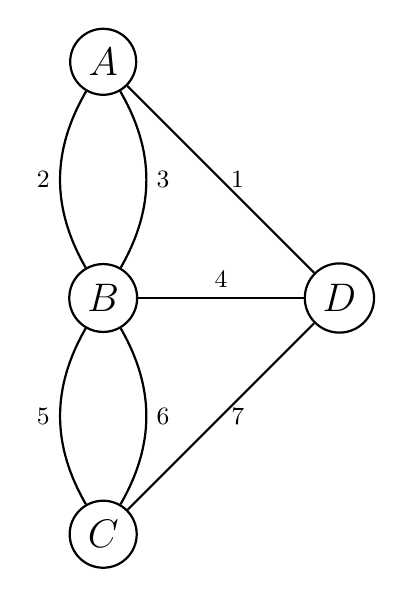
\begin{tikzpicture}[auto, node distance=3cm, every loop/.style={},
                    thick,main node/.style={circle,draw,font=\sffamily\Large\bfseries}]

  \node[main node] (1) {$A$};
  \node[main node] (2) [below of=1] {$B$};
  \node[main node] (3) [below of=2] {$C$};
  \node[main node] (4) [right of=2] {$D$};

  \path[every node/.style={font=\sffamily\small}]
    (1) edge node [right] {$1$} (4)
        edge [bend right] node[left] {$2$} (2)
    (2) edge [bend right] node [right] {$3$} (1)
        edge node {$4$} (4)
        edge [bend right] node[left] {$5$} (3)
    (3) edge [bend right] node [right] {$6$} (2)
    (4) edge node [right] {$7$} (3);
\end{tikzpicture}
\end{center}

It is worth noting two things about the above diagram. First that the labels on the vertices and edges are unrelated to the problem, but have been added simply to make referring to parts of the graph much easier. Second that whatever the above image depicts, does not fit our definition of a graph.

Notice that edge $2$ and edge $3$ both connect vertex $A$ to $B$, as well edges $5$ and $6$ do for $B$ and $C$. This is a strict violation of our definition for a graph. The issue of course then comes to what would one call such a beast as this where, presumably, one is able to have as many connections between any pair of vertices and could even have connections from a vertices to itself.

I am particularly glad that you're paying enough attention to notice that the diagram does not depict a graph. This is what we will refer to as a multigraph. It is worth noting that graphs are a type of multigraph, so anything we show to be true for all multigraphs, is also true for all graphs.

Now to solve this problem we need to make one simple observation about how we walk. If we are to go to island (or vertex) we must also leave that island, unless it is the last island we arrive on. This means, that with the exception of the island we start on and end on, each island must have an even number of bridges connected to it. On the multigraph we would say that we need all vertices but a start and end vertex to have an even number of edges. If we look at the multigraph above, we have four vertices that have an odd number of edges connected to them.

\subsection{History}
%TODO Make how short this is less obvious
The seven bridges of K\"onigsberg problem was solved by Euler %TODO Citation (wikipedia for seven bridges of konigsberg)
in 1736. In mathematics this problem is of great historical significance as it is considered to be the beginning of graph theory as well as a sort of precursor to topology. %TODO Citation 

\section{Graph Theory Background}

\subsection{Planer Graphs}

Consider the following graph.

\begin{center}
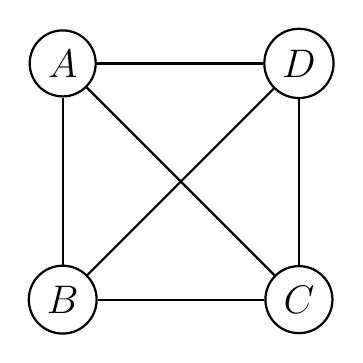
\begin{tikzpicture}[auto, node distance=3cm, every loop/.style={},
                    thick,main node/.style={circle,draw,font=\sffamily\Large\bfseries}]

  \node[main node] (1) {$A$};
  \node[main node] (2) [below of=1] {$B$};
  \node[main node] (3) [right of=2] {$C$};
  \node[main node] (4) [right of=1] {$D$};

  \path[every node/.style={font=\sffamily\small}]
    (1) edge node {} (4)
    	edge node {} (3)
    (2) edge node {} (1)
        edge node {} (4)
    (3) edge node {} (2)
    (4) edge node {} (3);
\end{tikzpicture}
\end{center}

This graph is called a complete as every vertex is connected to every other vertex by an edge; in fact this graph in particular is called $K_4$ as it is the complete four vertex graph. We would like to find out if we can draw this above graph without having any lines crossing. We can in fact draw this graph without any intersections and for any skeptics who may being reading this, the below is $K_4$ without any edges intersecting.

\begin{center}
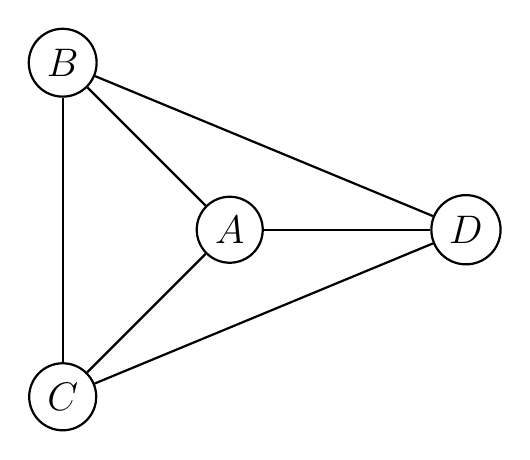
\begin{tikzpicture}[auto, node distance=3cm, every loop/.style={},
                    thick,main node/.style={circle,draw,font=\sffamily\Large\bfseries}]

  \node[main node] (1) {$A$};
  \node[main node] (2) [above left of=1] {$B$};
  \node[main node] (3) [below left of=1] {$C$};
  \node[main node] (4) [right of=1] {$D$};

  \path[every node/.style={font=\sffamily\small}]
    (1) edge node {} (4)
    	edge node {} (3)
    (2) edge node {} (1)
        edge node {} (4)
    (3) edge node {} (2)
    (4) edge node {} (3);
\end{tikzpicture}
\end{center}

So if this graph can be drawn without intersection, can any graph be drawn without intersections? If some can and some can't how do we tell which can be drawn and which can not? The answer to this comes in Kuratowski's theorem, however before we can even state this theorem we need to build up a bit of terminology for graph theory.

\subsection{Graph Drawing}
A graph drawing is exactly what it sounds like. We've already seen drawings of graphs like the one for K\"oingsberg and two drawings of $k_4$, this means there may be multiple distinct drawings for the same graph. Now we don't need to be very worried about what defines a drawing, that won't be important to us. Simply think of it as the drawing.

If a drawing has no edges intersecting it is said to be a plane drawing. If there exists such a drawing for a particular graph, then that graph is a planar graph.

\subsection{Face}
Faces are a bit of an odd property here as they fundamentally are actually properties only of plane drawings and not graphs themselves; however the number of faces, as we will see stays consistent between any plane drawing of a planar graph and as such the number of faces is a property that planar graphs have.

A face is defined as a connected space that contains no edges or vertices and itself is bounded by edges and vertices.

If you think back to high-school geometry and cubes you may recall that a each of the corners is a vertex, the lines connecting vertices are edges and the area between the edges are faces. In a graph we have vertices connected by edges and when we draw them there are empty areas enclosed by edges and vertices. For example the following would correspond with a cube
\begin{center}
	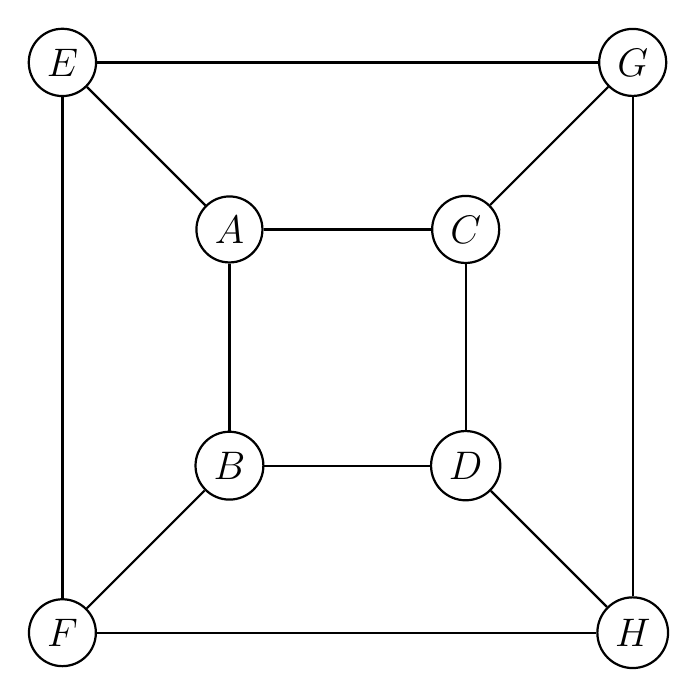
\begin{tikzpicture}[auto, node distance=3cm, every loop/.style={},
	thick,main node/.style={circle,draw,font=\sffamily\Large\bfseries}]
	
	\node[main node] (1) {$A$};
	\node[main node] (2) [below of=1] {$B$};
	\node[main node] (3) [right of=1] {$C$};
	\node[main node] (4) [right of=2] {$D$};
	\node[main node] (5) [above left of=1] {$E$};
	\node[main node] (6) [below left of=2] {$F$};
	\node[main node] (7) [above right of=3] {$G$};
	\node[main node] (8) [below right of=4] {$H$};
	
	\path[every node/.style={font=\sffamily\small}]
	(1) edge node {} (2)
	edge node {} (3)
	edge node {} (5)
	(2) edge node {} (4)
	edge node {} (6)
	(3) edge node {} (4)
	edge node {} (7)
	(4) edge node {} (8)
	(5) edge node {} (6)
	edge node {} (7)
	(6) edge node {} (8)
	(7) edge node {} (8);
	\end{tikzpicture}
\end{center}
Now we can imagine that if we look at the cube straight on maybe $ABDC$ would be the face we are looking at. So too we see the area enclosed in $ABDC$ is a face by the definition we gave. The same is true for $ABFE$, $ACGE$, $DBFH$, and $DCGH$, however that leaves us with only five faces on this cube. The last face must logically come from $EFHG$, however the area enclosed by that contains all the other edges and vertices, so it doesn't fit our definition. However we may notice that the infinite space outside $EFHG$ does not contain any vertices, and therefore we get a sixth face.

Consider then the following very simple graph:
\begin{center}
	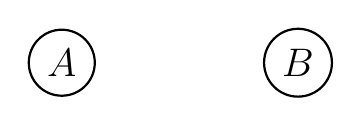
\begin{tikzpicture}[auto, node distance=3cm, every loop/.style={},
	thick,main node/.style={circle,draw,font=\sffamily\Large\bfseries}]
	
	\node[main node] (1) {$A$};
	\node[main node] (2) [right of=1] {$B$};
	
	
	\end{tikzpicture}
\end{center}
Now we still only have one face, however it doesn't have as nice a boundary as they did in the cube. However if we look at all of space excluding $A$ and $B$ then we still get a valid space by our definition.

\subsection{Walks}
Now moving onto a more traditional graph property we have the concept of a walk. A walk can be thought of as if you were standing on some vertex $v_0$ and just kept following edges to neighboring vertices some number of times. We define it as follows.

\begin{definition}[walk]
	A walk is a finite sequence of vertices and edges with the following properties.
	\begin{itemize}
		\item Every odd element in the sequence is a vertex.
		\item Every even element in the sequence is an edge that connects the vertex before and after it.
		\item A walk always begins and ends with a vertex.
	\end{itemize}
\end{definition}

For example consider the following graph.

\begin{center}
	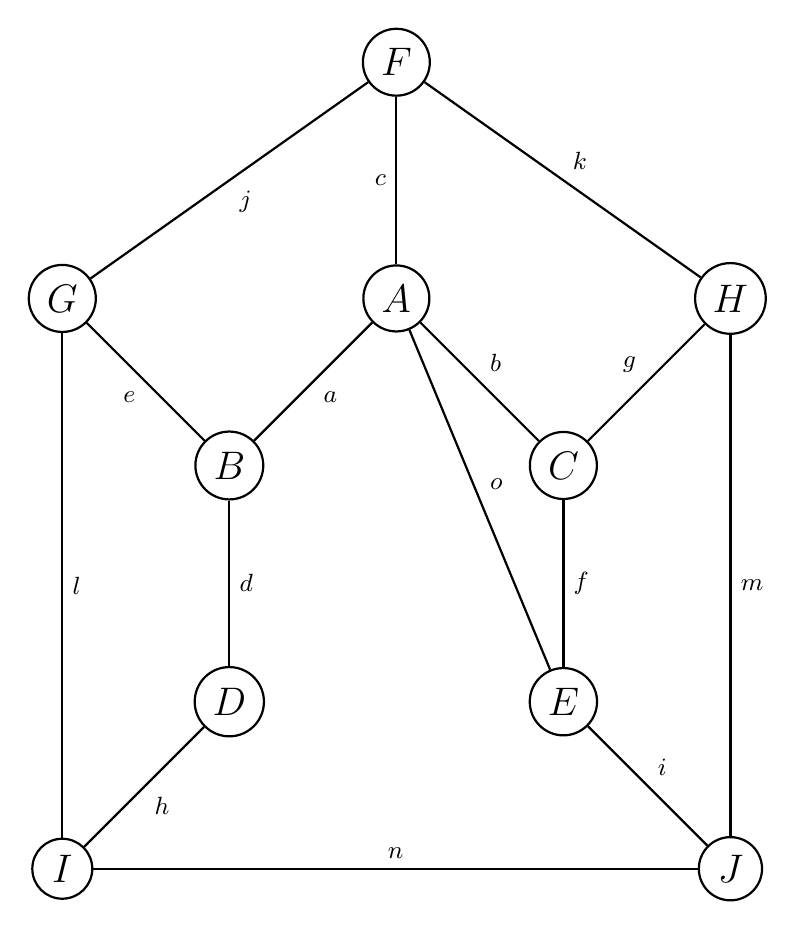
\begin{tikzpicture}[auto, node distance=3cm, every loop/.style={},
	thick,main node/.style={circle,draw,font=\sffamily\Large\bfseries}]
	
	\node[main node] (a) {$A$};
	\node[main node] (b) [below left of=a] {$B$};
	\node[main node] (c) [below right of=a] {$C$};
	\node[main node] (d) [below of=b] {$D$};
	\node[main node] (e) [below of=c] {$E$};
	\node[main node] (f) [above of=a] {$F$};
	\node[main node] (g) [above left of=b] {$G$};
	\node[main node] (h) [above right of=c] {$H$};
	\node[main node] (i) [below left of=d] {$I$};
	\node[main node] (j) [below right of=e] {$J$};
	
	\path[every node/.style={font=\sffamily\small}]
	(a) edge node {$a$} (b)
	edge node {$b$} (c)
	edge node {$c$} (f)
	edge node {$o$} (e)
	(b) edge node {$d$} (d)
	edge node {$e$} (g)
	(c) edge node {$f$} (e)
	edge node {$g$} (h)
	(d) edge node {$h$} (i)
	(e) edge node {$i$} (j)
	(f) edge node {$j$} (g)
	edge node {$k$} (h)
	(g) edge node {$l$} (i)
	(h) edge node {$m$} (j)
	(i) edge node {$n$} (j);
	\end{tikzpicture}
\end{center}

Now the sequence $BeGjF$ is a walk as we can think of starting at vertex $B$, walking down $e$ to $G$, then down $j$ to $F$ and  finishing. The sequence $AaBaA$ is also a walk as we could start at $A$, go down edge $a$ to $B$, then back up $a$ to $A$ again. The sequence $CfEi$ however isn't a walk as it doesn't end with a vertex. 

\subsubsection{Path}
\begin{definition}[path]
	A path is a walk where a vertex and edge can not appear twice in the sequence.
\end{definition}
 
You could think of a path as you start at some vertex and start building a path as you talk your walk. You aren't allows to have your path intersect with itself, so you always 
 
So for example with the above graph $BeGjF$ is not only a walk, but also a path. The sequence $AaBaA$, while it is a walk, it however is not a path as both edge $a$ and vertex $A$ are used twice.

\subsubsection{Cycle}
\begin{definition}[cycle]
	A cycle is a walk, of length greater than one, where a vertex and edge can not appear twice in the sequence with the exception of the first and last vertex which must be the same.
\end{definition}


The definition for cycle is quite similar to that of a path, it effectively is a path that loops back to where it started at the end. The stipulation that a cycle must be "of length greater than one" simply means that the walk $A$ (just the vertex $A$ and nothing else) is not a cycle. Examples of a cycle would include $AbCgHkFcA$, $AbCfEoA$, and $FkHmJnIlGjF$. It is important to note that something like $FcAcF$ is not a cycle as it includes the edge $c$ twice.

\subsection{Connected}
A graph is said to be connected if for any pair of vertices, $\pair ab$ there is a walk from $a$ to $b$. So if we consider the following graphs 
\begin{center}
	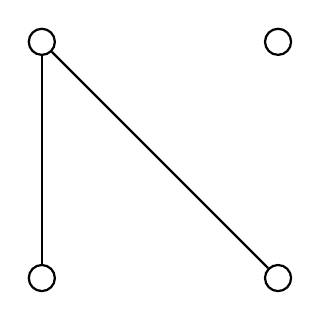
\begin{tikzpicture}[auto, node distance=3cm, every loop/.style={},
	thick,main node/.style={circle,draw,font=\sffamily\Large\bfseries}]
	
	\node[main node] (1) {};
	\node[main node] (2) [right of=1] {};
	\node[main node] (3) [below of=1] {};
	\node[main node] (4) [right of=3] {};
	
	\path[every node/.style={font=\sffamily\small}]
	(1)	edge node {} (3)
	(4) edge node {} (1);
	\end{tikzpicture}\quad\quad\quad
	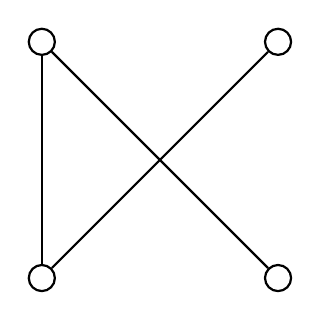
\begin{tikzpicture}[auto, node distance=3cm, every loop/.style={},
	thick,main node/.style={circle,draw,font=\sffamily\Large\bfseries}]
	
	\node[main node] (1) {};
	\node[main node] (2) [right of=1] {};
	\node[main node] (3) [below of=1] {};
	\node[main node] (4) [right of=3] {};
	
	\path[every node/.style={font=\sffamily\small}]
	(1)	edge node {} (3)
	(2) edge node {} (3)
	(4) edge node {} (1);
	\end{tikzpicture}\quad\quad\quad
	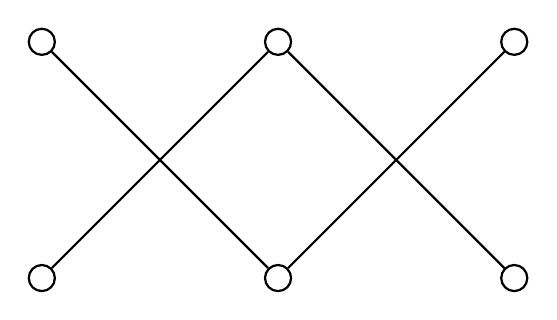
\begin{tikzpicture}[auto, node distance=3cm, every loop/.style={},
	thick,main node/.style={circle,draw,font=\sffamily\Large\bfseries}]
	
	\node[main node] (1) {};
	\node[main node] (2) [right of=1] {};
	\node[main node] (3) [right of=2] {};
	\node[main node] (4) [below of=1] {};
	\node[main node] (5) [right of=4] {};
	\node[main node] (6) [right of=5] {};
	
	\path[every node/.style={font=\sffamily\small}]
	(1)	edge node {} (5)
	(2) edge node {} (4)
	edge node {} (6)
	(3) edge node {} (5);
	\end{tikzpicture}
\end{center}
We find that only the graph in the middle is connected. For the graph on the right consider any vertex on the bottom, there is no path to the vertex above it. The graph on the left is has the upper right vertex isolated from the rest of the graph.

Any graph, connected or not, can be broken into connected components. To do this we simply take a vertex and every other vertex connected to it and call that one component, and then repeat with a vertex not in that component. This sort of breaking apart is nice as often we will prove things about connected graphs that are true about all graphs. For example if all components of a graph are planar then the entire graph must be planar, this will be proven below and it allows us to only deal with connected graphs.

%\subsection{Neighborhood}
%Given some graph $G$ with vertex $v$. The neighborhood of $v$ within $G$ is the set of all vertices that share an edge with $v$, not including $v$.\footnote{If $G$ is a multigraph the definition stays the same, however $v$ maybe its own neighbor if it has an edge with itself or a loop} Given a subgraph $H$ of $G$, the neighborhood of $H$ within $G$ is a new subgraph of $G$ that includes $H$ as well as any vertex in $G$ that is adjacent to a vertex in $H$ and the edge that they share.
%
%Lets look at some examples
%\begin{center}
%	\begin{tikzpicture}[auto, node distance=3cm, every loop/.style={},
%	thick,main node/.style={circle,draw,font=\sffamily\Large\bfseries}]
%	
%		\node[main node] (0) {\textcolor{blue}{$a$}};
%		\node[main node] (1) [above right of=0] {\textcolor{red}{$b$}};
%		\node[main node] (2) [right of=1] {$c$};
%		\node[main node] (3) [below right of=2] {$d$};
%		\node[main node] (4) [below of=3] {\textcolor{red}{$e$}};
%		\node[main node] (5) [below left of=4] {$f$};
%		\node[main node] (6) [left of=5] {$g$};
%		\node[main node] (7) [above left of=6] {$h$};
%		
%		\path[every node/.style={font=\sffamily\small}]
%		(0)
%		edge node {} (2)
%		edge node {} (3)
%		edge node {} (4)
%		(1)
%		edge node {} (3)
%		edge node {} (4)
%		edge node {} (5)
%		(2)
%		edge node {} (4)
%		edge node {} (5)
%		(3)
%		edge node {} (7)
%		(4)
%		edge node {} (6)
%		edge node {} (7)
%		(5)
%		edge node {} (6)
%		edge node {} (7)
%		(6)
%		edge node {} (7);
%	\end{tikzpicture}
%\end{center}
%
%First let us consider the neighborhood of just the vertex \textcolor{blue}{$a$}, this would then be all the vertices that it is adjacent to so we get $$\set{c, d, \textcolor{red}{e}}$$ We could also let $A$ be a subgraph containing only the vertex $\textcolor{blue}{a}$ and so its neighborhood within $G$ will be the graph below.
%\begin{center}
%	\begin{tikzpicture}[auto, node distance=3cm, every loop/.style={},
%	thick,main node/.style={circle,draw,font=\sffamily\Large\bfseries}]
%	
%		\node[main node] (0) {\textcolor{blue}{$a$}};
%		\node[main node] (2) [above right of=0] {$c$};
%		\node[main node] (3) [below right of=2] {$d$};
%		\node[main node] (4) [below of=3] {\textcolor{red}{$e$}};
%		
%		\path[every node/.style={font=\sffamily\small}]
%		(0)
%		edge node {} (2)
%		edge node {} (3)
%		edge node {} (4)
%		(2)
%		edge node {} (4);
%	\end{tikzpicture}
%\end{center}
%The difference is that this is actually a subgraph of $G$, whereas the previous is just vertices.
%
%For another example let $H$ be the subgraph with only the \textcolor{red}{$b$}, \textcolor{red}{$e$} and the edge they share. The neighborhood of $H$ within $G$ within $G$ would then be all of $G$ as every vertex is either a neighbor of $b$ or $e$.
%
\subsection{Contraction}

\subsubsection{Edge contraction}
This is not a property, but rather an operation or action that we perform on a graph. Let us consider the following graph.

\begin{center}
	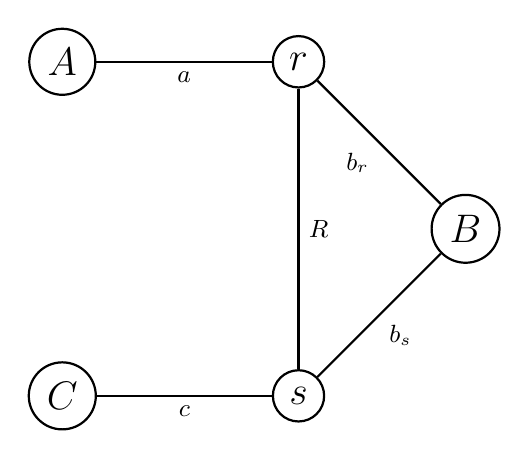
\begin{tikzpicture}[auto, node distance=3cm, every loop/.style={},
	thick,main node/.style={circle,draw,font=\sffamily\Large\bfseries}]
	
	\node[main node] (1) {$r$};
	\node[main node] (2) [below right of=1] {$B$};
	\node[main node] (3) [left of=1] {$A$};
	\node[main node] (4) [below left of=2] {$s$};
	\node[main node] (5) [left of=4] {$C$};
	
	\path[every node/.style={font=\sffamily\small}]
	(1) edge node {$R$} (4)
	edge node {$a$} (3)
	(2) edge node {$b_r$} (1)
	edge node {$b_s$} (4)
	(4) edge node {$c$} (5);
	\end{tikzpicture}
\end{center}

We wish to perform a contraction on edge $R$. To be clear all graph contractions are on edges. So we will make a new vertex, $r\cdot s$ which has all the edges of $r$ and all the edges of $s$ except the edge we are contracting across. In this case the edge we are contracting across is $R$ and thus we get the following multigraph.

\begin{center}
	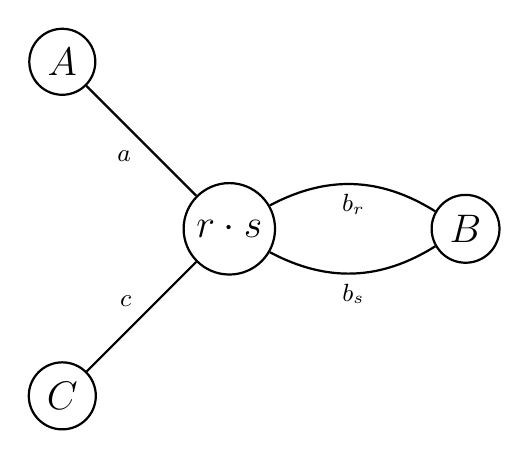
\begin{tikzpicture}[auto, node distance=3cm, every loop/.style={},
	thick,main node/.style={circle,draw,font=\sffamily\Large\bfseries}]
	
	\node[main node] (1) {$r\cdot s$};
	\node[main node] (2) [right of=1] {$B$};
	\node[main node] (3) [above left of=1] {$A$};
	\node[main node] (4) [below left of=1] {$C$};
	
	\path[every node/.style={font=\sffamily\small}]
	(1)	edge node {$a$} (3)
	(2) edge [bend right] node {$b_r$} (1)
	edge [bend left] node {$b_s$} (1)
	(4) edge node {$c$} (1);
	\end{tikzpicture}
\end{center}

Often we may prefer to have the end result be a graph rather than a multigraph, which brings us to our next kind of contraction

\subsubsection{Simple edge contraction}

We can take any multigraph produced by an edge contraction and for any edge pairs that go between the same vertices, simply replace it with a single edge. This will reduce the multigraph back to a graph, and from the previous example the result of a simple edge contraction on $R$ will give the below graph.

\begin{center}
	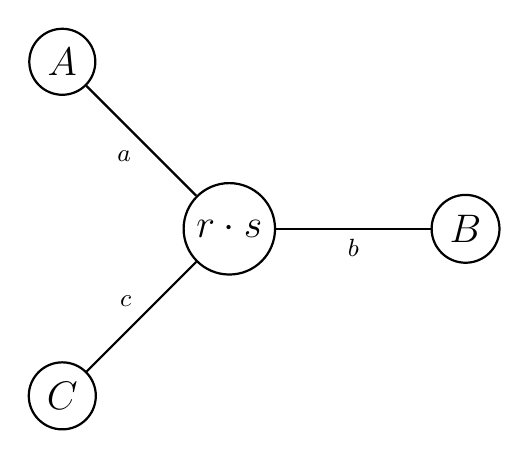
\begin{tikzpicture}[auto, node distance=3cm, every loop/.style={},
	thick,main node/.style={circle,draw,font=\sffamily\Large\bfseries}]
	
	\node[main node] (1) {$r\cdot s$};
	\node[main node] (2) [right of=1] {$B$};
	\node[main node] (3) [above left of=1] {$A$};
	\node[main node] (4) [below left of=1] {$C$};
	
	\path[every node/.style={font=\sffamily\small}]
	(1)	edge node {$a$} (3)
	(2) edge node {$b$} (1)
	(4) edge node {$c$} (1);
	\end{tikzpicture}
\end{center}

%\subsection{Subdivision}
%There are two types of subdivision, an edge subdivision and graph subdivision. Edge subdivisions can best be though of as an operation, much like a contraction. We then can define a graph subdivision in terms of the edge version.

%\subsubsection{Edge Subdivision}
%An edge subdivision is where we take an an edge and add a vertex into the middle of it. If we have an edge $e$ that goes between vertex $a$ and $b$ then to subdivide it we add a vertex $c$, remove edge $e$ and then add an edge between $a$ and $c$ and between $b$ and $c$. This is demonstrated in the diagram below.
%\begin{center}
%	$
%	\begin{array}{l}
%		\begin{tikzpicture}[auto, node distance=3cm, every loop/.style={},
%		thick,main node/.style={circle,draw,font=\sffamily\Large\bfseries}]
%		
%			\node[main node] (1) {$a$};
%			\node[main node] (2) [right of=1] {$b$};
%			
%			\path[every node/.style={font=\sffamily\small}]
%			(1)	edge node {$e$} (2);
%		\end{tikzpicture}
%	\end{array}
%	$
%	\scalebox{2}{$\to$}
%	$
%	\begin{array}{l}
%		\begin{tikzpicture}[auto, node distance=3cm, every loop/.style={},
%thick,main node/.style={circle,draw,font=\sffamily\Large\bfseries}]
%
%		\node[main node] (1) {$a$};
%		\node[main node] (3) [right of=1] {$c$};
%		\node[main node] (2) [right of=3] {$b$};
%		
%		\path[every node/.style={font=\sffamily\small}]
%		(1)	edge node {} (3)
%		(2) edge node {} (3);
%		\end{tikzpicture}
%	\end{array}
%	$
%\end{center}
%
%This can be thought of as a sort of inverse to contractions. To see this simply perform a contraction on either edge of the output graph above and you will return the the original graph.
%
%
%\subsubsection{Graph Subdivision}
%A graph $G$ is said to be a subdivision of $H$ if $G$ can be obtained from $H$ via some series of edge subdivisions. For example consider the two following graphs.
%This can be thought of as just adding vertices along an edge. Intuitively this shouldn't actually change the shape of a graph. This not changing the shape of a graph is something that will be touched on later in lemma \ref{subdivision}.

\section{Kuratowski's Theorem}
\begin{restatable}[Kuratowski]{theorem}{THEBIGONE}\label{THEBIGONE}
	A graph $G$ is nonplanar if and only if it contains a subgraph that is a subdivision of $K_{3,3}$ or $K_5$
\end{restatable}

%TODO Maybe explanation of what $K_5$ and $K_{3,3}$ are should be earlier?
Here $K_5$ refers to the complete graph on 5 vertices, and $K_{3,3}$ is the complete bipartite graph with three vertices in both partitions. Drawings of both theses graphs are below with ($K_5$ on left and $K_{3,3}$ on right).
\begin{center}
	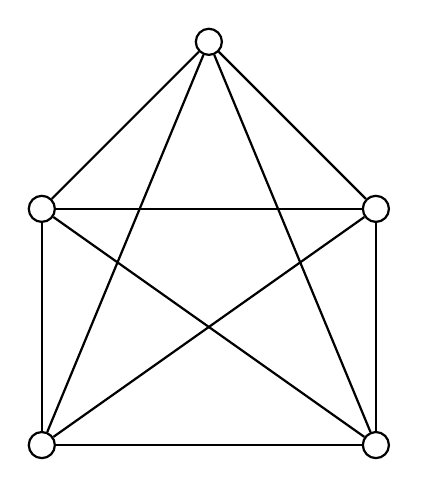
\begin{tikzpicture}[auto, node distance=3cm, every loop/.style={},
	thick,main node/.style={circle,draw,font=\sffamily\Large\bfseries}]
	
	\node[main node] (1) {};
	\node[main node] (2) [below left of=1] {};
	\node[main node] (3) [below right of=1] {};
	\node[main node] (4) [below of=2] {};
	\node[main node] (5) [below of=3] {};
	
	\path[every node/.style={font=\sffamily\small}]
	(1)	edge node {} (2)
	edge node {} (3)
	edge node {} (4)
	edge node {} (5)
	(2) edge node {} (3)
	edge node {} (4)
	edge node {} (5)
	(3) edge node {} (4)
	edge node {} (5)
	(4) edge node {} (5);
	\end{tikzpicture}
	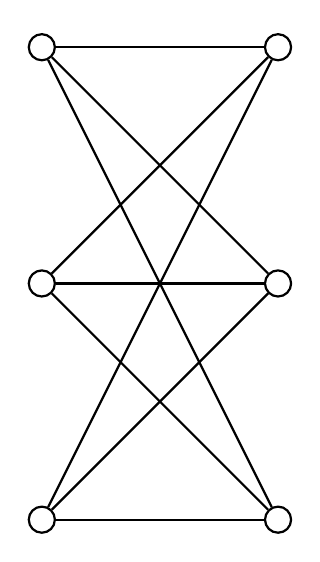
\begin{tikzpicture}[auto, node distance=3cm, every loop/.style={},
	thick,main node/.style={circle,draw,font=\sffamily\Large\bfseries}]
	
	\node[main node] (1) {};
	\node[main node] (2) [below of=1] {};
	\node[main node] (3) [below of=2] {};
	\node[main node] (4) [right of=1] {};
	\node[main node] (5) [below of=4] {};
	\node[main node] (6) [below of=5] {};
	
	\path[every node/.style={font=\sffamily\small}]
	(1)	edge node {} (4)
	edge node {} (5)
	edge node {} (6)
	(2)	edge node {} (4)
	edge node {} (5)
	edge node {} (6)
	(3)	edge node {} (4)
	edge node {} (5)
	edge node {} (6);
	\end{tikzpicture}
\end{center}

\subsection{$K_5$ and $K_{3,3}$}
Our first step is proving that $K_{3,3}$ and $K_5$ are nonplanar. To do this we are going to use the following theorem.

\begin{theorem}[Euler's formula on planar multigraphs]
	For any plane drawing of a multigraph (with the exception of a multigraph with no vertices), we have $$v-e+f=2$$, where $v$ is the number of vertices in the multigraph, $e$ is the number of edges in the multigraph, and $f$ is the number of faces in the plane drawing of the multigraph.
\end{theorem}

%TODO cite https://www.ics.uci.edu/~eppstein/junkyard/euler/iedge.html


\begin{proof}
	First consider a connected multigraph with no edges, as this is connected we may only have a single vertex. This produces a single and no edges so we find $$v-e+f=1-0+1=2$$ Now that we know that for 0 edges this rule fits, then either the rule ($v-e+f-2$) is true no mater the number of edges, or there is some number at which point this rule breaks, and $v-e+f\not=2$. If there is a number that breaks this rule, then there must be a lowest number (let's call it $k$) that breaks this rule. For any multigraph with $k$ edges, choose any edge $e$ in the graph.
	\begin{itemize}
		\item If $e$ connects a vertex to itself it is a loop and its removal will result in the loss of one edge and one face (each loop creates a face\footnote{this is due to the Jordan curve theorem}). The resulting multigraph has less than $k$ edges and thus we know that for it \begin{align*}2&=v-e+f \\&= v-(e+1)+(f+1)\end{align*} and as the original graph had one more edge and one more face it too would fit this rule.
		\item If $e$ is not a loop we may perform an edge contraction on it and this will reduce both the number of edges and the number of vertices by one. Again this gives us a multigraph with less than $k$ edges so we know that for it \begin{align*}2&=v-e+f\\&=(v+1)-(e+1)+f\end{align*} and as the original graph had one more edge and one more vertex it to would fit this rule.
	\end{itemize}
	
	From this we know that there can not possibly be some $k$, and thus all multigraphs, regardless of the number of edges must fit this rule.
\end{proof}
This leads to a nice corollary, that will be helpful when talking about graphs.
\begin{corallary}
	Any plane drawing of any multigraph has the same number of faces.
\end{corallary}
\begin{proof}
	Any planar multigraph can be broken into connected components. Each component of a planar multigraph is a connected planar multigraph and thus any planar drawing of it fits the rule $v-e+f=2$.  Now any plane drawing we make of a planar multigraph will be made of parts that already have a constant number of faces.\footnote{This is not a complete proof, to complete it you simply make an induction on the number of components drawn and realize each time you add a component you add exactly $f_{i}-1$ new faces (if $f_i$ is the number of faces in the $i^{\text{th}}$ component drawn).}
	
	%Each drawing of every component has the same number of edges and vertices, and therefore by our equation the number of faces must also be the same in each component's drawing. Now we make a plane drawing of each component one by one to create a plane drawing of the full multigraph. Choose a component to draw first and when we draw it we know it will have some number $f_1$ of faces regardless of its drawing. Now if we have already drawn in $k$ components we can add the $k+1^{\text{th}}$ component. To do this we must draw it completely within one of the faces that already exists as it is a plane drawing. This adds exactly $f_{k+1}-1$ faces by drawing this component as it simply splits one already existing face into $f_{k+1}$ new faces. This means that no mater what order we add faces in 
\end{proof}

This means that given any planar multigraph $G$, we can talk about the number of faces $G$ has without referring to any drawing of $G$, as all plane drawings will have the same number of faces.

Now using this we can prove that $K_{3,3}$ and $K_5$ are nonplanar.

\begin{theorem}
	$K_5$ is nonplanar.
\end{theorem}
\begin{center}
	\scalebox{.6}{
		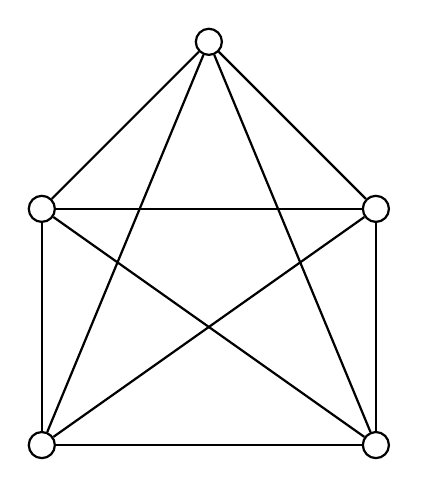
\begin{tikzpicture}[auto, node distance=3cm, every loop/.style={},
		thick,main node/.style={circle,draw,font=\sffamily\Large\bfseries}]
		
			\node[main node] (1) {};
			\node[main node] (2) [below left of=1] {};
			\node[main node] (3) [below right of=1] {};
			\node[main node] (4) [below of=2] {};
			\node[main node] (5) [below of=3] {};
			
			\path[every node/.style={font=\sffamily\small}]
			(1)	edge node {} (2)
			edge node {} (3)
			edge node {} (4)
			edge node {} (5)
			(2) edge node {} (3)
			edge node {} (4)
			edge node {} (5)
			(3) edge node {} (4)
			edge node {} (5)
			(4) edge node {} (5);
		\end{tikzpicture}
	}

	\scalebox{.9}{$K_5$}
\end{center}
\begin{proof}
	$K_5$ is a graph\footnote{Recall that all graphs are multigraphs, but not all multigraphs are graphs.}, and as such an edge can not be a loop and two vertices can share at most one edge. This means that in any plane drawing of a graph, there must be at least 3 edges bordering every face.
	\begin{itemize}
		\item To only have one edge bordering a face would require that the edge be a loop (which we can't have in a graph).
		\item To only have only two edges bordering a face would require that some pair of vertices share more than one edge (which we can't have in a graph).
	\end{itemize}
	Additionally every edge borders no more than two faces, so from this we know that in any graph $2e \ge 3f$ or $\frac23e\ge f$. Now $K_5$ has 10 edges and 5 vertices, so we know that $$\frac2310=\frac{20}3=6.\bar6\ge f$$ We know that $K_5$ is a connected graph (and thus also a connected multigraph) so if $K_5$ were planar then we would have $$2=v-e+f=5-10+f\le5-10+6.\bar6 = 1.\bar6$$ which is clearly false as $$2\not\le1.\bar6$$ Therefore $K_5$ must not be planar.
\end{proof}

\begin{theorem}
	$K_{3,3}$ is nonplanar.
\end{theorem}
\begin{center}
	\scalebox{.6}{
		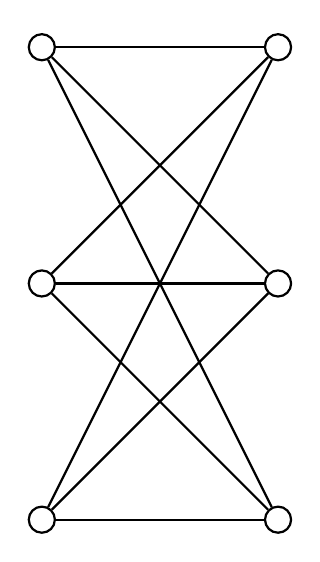
\begin{tikzpicture}[auto, node distance=3cm, every loop/.style={},
		thick,main node/.style={circle,draw,font=\sffamily\Large\bfseries}]
	
			\node[main node] (1) {};
			\node[main node] (2) [below of=1] {};
			\node[main node] (3) [below of=2] {};
			\node[main node] (4) [right of=1] {};
			\node[main node] (5) [below of=4] {};
			\node[main node] (6) [below of=5] {};
			
			\path[every node/.style={font=\sffamily\small}]
			(1)	edge node {} (4)
			edge node {} (5)
			edge node {} (6)
			(2)	edge node {} (4)
			edge node {} (5)
			edge node {} (6)
			(3)	edge node {} (4)
			edge node {} (5)
			edge node {} (6);
		\end{tikzpicture}
	}
		
	\scalebox{.9}{$K_{3,3}$}
\end{center}
\begin{proof}
	$K_{3,3}$ is a bipartite graph, meaning that there is some way to break the graph into two collections of vertices, where there are no edges that stay within one of these collections. If we look at the drawing of $K_{3,3}$ above we see that the right and left works as these collections for us. There is no edge that goes between two vertices on the right or two vertices on the left. This means that if we can make a plane drawing of $K_{3,3}$ each face must have at least four edges on its boundary. We know from our proof of $K_5$'s nonplanarity that each face in a graph must have at least three edges on its boundary. If any face were to have three edges then the cycle bounding the face would have exactly three vertices as well. Each pair of vertices within these three vertices would share an edge and therefore there is no way to split them up into two groups such that neither group has an edge within it. Additionally every edge borders no more than two faces, so from this we know that in any bipartite graph $2e \ge 4f$ or $e\ge 2f$.
	
	Now $K_{3,3}$ has 6 vertices and 9 edges. $K_{3,3}$ is bipartite so the number of faces, $f \le \frac e2 = \frac92 = 4.5$. $K_{3,3}$ is connected, so if it were planar we would have Euler's formula giving us $$2=v-e+f=6-9+f\le6-9+4.5=1.5$$ and this is false as $$2\not\le1.5$$ Therefore $K_{3,3}$ is nonplanar.
\end{proof}

\subsection{Drawings}
Up to this point the paper has been writing such that anyone with a basic mathematical competency and interest could understand and work through the content. From this point on the paper moves a bit faster and assumes knowledge of basic mathematical notation and more experience with math.

The purpose of the next couple sections is to build up the mathematical machinery that we need for our proof of Kuratowski's theorem (theorem \ref{THEBIGONE}). In this section we will be proving a slew of lemmas and theorems, as well as provide a couple definitions, all of which will be needed in our final proof.

We start by going back and formalizing our idea of a graph drawing. All this is meant to do is use mathematical language to define what we have already been thinking of as a graph drawing.

\begin{definition}[Drawing]
	A drawing is a subset, $D$, of some topological space $S$. For plane drawings this space will be $\mathbb R^2$ with its standard topology.
\end{definition}

\begin{definition}[Graph Drawing]
Given a graph $G$, with vertex set $V$ and edge set $E$, a drawing $D$ is said to be a drawing of $G$ if and only if the following criteria are met:
\begin{itemize}
	\item There exists an injective function $v:V\to D$.
	\item If there is an edge $e\in E$ between vertices $a$ and $b$ then there is a continuous injective function $\hat e:\ccint01\to S$ with $\hat e(0) = v(a)$ and $\hat e(1) = v(b)$ and the image of $e$ is contained within $D$.\footnote{In a multigraph drawing we may have $a=b$ and thus $\hat e(0) = \hat e(1)$ making $\hat e$ not injective, however it must still be injective in $\coint 01$.}
	\item For any vertex $a\in V$ and edge $e\in E$ and any real number $x\in\ooint 01$, $\hat e(x)\not=v(a)$.
	\item For any two edges $e\not=f$, $\hat e(x) \not= \hat f(y)$ for all $x,y \in\ooint01$.
	\item for all $d\in D$ there exists either a vertex $a\in V$ such that $v(a) = d$ or there exists an edge $e\in E$ such that $d$ is in the image of $\hat e$.
\end{itemize}
\end{definition}


\subsection{Subgraph lemmas}

\begin{lemma} \label{subgraph}
	If a graph $G$ has a nonplanar subgraph, then $G$ is nonplanar.
\end{lemma}

\begin{proof}
	If we have a graph $G$ with a nonplanar subgraph $H$ then when drawing $G$ there is a part of the drawing that is $H$. This part of the drawing can not be planar and therefore the drawing of $G$ can not be a plane drawing.
\end{proof}

\begin{definition}[contactable]
	A graph $G$ is said to be contactable to a graph $H$ if there is some series of simple edge contractions that when performed on $G$ produce $H$.
\end{definition}

\begin{lemma}
	If a graph $G$ with edge $e$ is planar then so is the graph produced by performing a simple edge contraction on $e$.
\end{lemma}

\begin{proof}
	Let $G$ be a planar graph with edge $e$ between $x$ and $y$. et $G'$ be the graph produced by an edge contraction on $e$. We are going to prove this using induction on the number of edges of $y$.
	
	Statement: $G'$ is planar and there is a plane drawing of $G'$ where all vertices, $v$, that border a face that $y$ borders in $G$ also a face that $x\cdot y$ borders in $G'$ ($x\cdot y$ is the vertex produced by contracting across $e$).
	
	Base case: Suppose $y$ only has edge $e$. Clearly $G'\subset G$ so by lemma \ref{subgraph} $G'$ must be planar. Additionally as $y$ has only one edge it can not possibly lie upon any cycles in $G$, this means that $y$ can only border at most 1 face, and as it has an edge to $x$ it must share this face with $x$. We may draw $G'$ simply be removing $e$ and $y$ from any drawing of $G$ and relabeling $x$ as $x\cdot y$. Clearly then the statement above must be true when $y$ has only one edge.
	
	Inductive step: Let $z\not=x$ be a vertex sharing edge $\bar e$ with $y$. Assume that the statement is true in $G\setminus\set{\bar e}$. Now perform a contraction on $e$ in $G\setminus\set{\bar e}$ to produce $H$. $x\cdot y$ in $H$ must border a face $\bar f$ that $z$ borders so we may add in edge $\bar e$ to $H$ in face $\bar f$ and produce a plane drawing of $G'$. Further let $v$ be a vertex bordering a face $f$ in $G$ that $y$ also borders. We then know that there is a face $f'$ in $H$ that borders both $v$ and $x \cdot y$. If $f'\not=\bar f$ then clearly $x\cdot y$ and $v$ both boarder $f'$ in $G'$ as well as $H$. If $f'=\bar f$ then $f'$ is split into two parts by $\bar e$ in $G'$, both of which are bordered by $x\cdot y$. Therefore our statement must be true for $G$.
	
	Now by induction we have proven the statement is true on all graphs and therefore our lemma is proved.
\end{proof}

\begin{corallary} \label{contractible}
	If a graph $G$ is planar, and if $G$ is contactable to a graph $H$, then $H$ must also be planar.
\end{corallary}

\begin{proof}
	Let $c_1,c_2,\ldots, c_n$ be the sequence of contractions on $G$ that produce $H$. Let $H_i$ be the graph produced after the first $i$ contractions on $G$, so $H_i = G$ and $H_n = H$. If $G$ is planar then clearly $H_0$ is planar. If $H_i$ is planar, then by the above lemma clearly $H_{i+1}$ is planar. Now by induction, if $G$ is planar $H$ must be planar.
\end{proof}

\begin{lemma} \label{contractibleCarryOn}
	If a graph $G$ has a subgraph that is contactable to $H$ as a subgraph, then graph $G'$ that is contactable to $G$ also contains a subgraph that is contactable to $H$.
\end{lemma}

\begin{proof}
		Let $H$ be a graph. Let $H'$ be contactable to $H$. Let $G$ be a graph that contains $H'$ as a subgraph. Let $G'$ be a graph that is contactable to $G$. There is some sequence of simple edge contractions $h_1,h_2,\ldots,h_\ell$ that produce $H$ from $H'$ as is there some sequence of simple edge contractions $g_1,g_2,\ldots,g_m$ that produce $G$ from $G'$.
		If we reverse these sequences we get sequences of inverse simple edge contractions that take produce $H'$ from $H$ and $G'$ from $G$. Each inverse simple edge contraction will be done on a single vertex (and turn it into two vertices that share an edge). Let $f_i = h_{\ell-i+1}$ and $e_i = g_{i-m+1}$ so that they are the reversed sequences of $g$ and $h$. Take the subsequence, $e_{i_1},e_{i_2},\ldots,e_{i_n}$ that consists of all the inverse simple edge contractions that act on a vertex within the subgraph $H'$ of $G$. Now we can produce $H''$ as the graph produced by performing the following inverse simple edge contractions on $H$
		$$ f_1,f_2,\ldots,f_\ell,e_{i_1},e_{i_2},\ldots,e_{i_n} $$
		Clearly now $H''$ is contactable to $H$ and $H''$ must be a subgraph of $G'$.
\end{proof}

%%TODO remove?
%\begin{lemma} \label{subdivision}
%	If a graph $G$ is a subdivision of a nonplanar graph, then $G$ is nonplanar.
%\end{lemma}
%
%\begin{proof}
%	Let $H$ be a nonplanar graph with edge, $e$, between vertices $a$ and $b$. Let $H'$ be the graph produced by performing an edge subdivision on edge $e$. Let us call the new call the new vertex $v$ and the new edges $e_a$ and $e_b$ ($e_a$ is an edge from $a$ to $v$ and $e_b$ is an edge from $b$ to $v$).
%	
%	Suppose there exists a plane drawing, $D$, of $H'$. Then there are continuous injective functions $\hat e_a,\hat e_b\ccint01\to\mathbb R^2$ with $\hat e_a(1) = \hat e_b(0)$ whose range is contained in $D$. Additionally we know that $\hat e_a(x) \not= \hat e_b(y)$ for any $x,y\in\ooint 01$. Further we know that $a\not=b$ as otherwise $H$ would be a multigraph with $e$ being a loop in it. This means that $v(a) = \hat e_a(0) \not= \hat e_b(x)$ and $v(b) = \hat e_b(1)\not=\hat e_a(x)$ for all $x\in\ccint 01$. With all this we can construct an continuous injective function $\hat e:\ccint01\to \mathbb R^2$ such that $\hat e(0) = a$ and $\hat e(1) = b$ with 
%	$$\hat e(x) = \begin{cases}
%	\hat e_a(x*2) & x \le \frac12\\
%	\hat e_b(x*2-1) & x > \frac 12
%	\end{cases}$$
%	As both $\hat e_a$ and $\hat e_b$ map into $D$, then so must $\hat e$ map into $D$. This contradicts our original statement that $H$ is nonplanar, and therefore $H'$ must not have a plane drawing.
%	
%	It follows by induction that if a graph is a subdivision of a nonplanar graph, that graph must be nonplanar.
%\end{proof}


\begin{lemma} \label{component}
	If a graph $G$ is nonplanar than at least one of its connected components is nonplanar.
\end{lemma}

\begin{proof}
	Suppose there exists a nonplanar graph $G$ for which all of its components are planar. If each component is planar we may also make a drawing of it in any space homeomorphic to $\mathbb R^2$. Simply embed each component in a separate open epsilon ball about an integer point, with $\varepsilon \le \frac12$, and we find a contradiction with a planar embedding of $G$.
\end{proof}

%%TODO remove?
%\begin{lemma} \label{subdivisionCarryOn}
%	If a graph $G$ has a subdivision of $H$ as a subgraph, then any subdivision of $G$ contains a subdivision of $H$ as a subgraph.
%\end{lemma}
%\begin{proof}
%	Let $H$ be a graph. Let $H'$ be a subdivision of $H$. Let $G$ be a graph that contains $H'$ as a subgraph. Let $G'$ be a subdivision of $G$. There is some sequence of edge subdivisions $h_1,h_2,\ldots,h_\ell$ that produce $H'$ from $H$ as is there some sequence of edge subdivisions $g_1,g_2,\ldots,g_m$ that produce $G'$ from $G$. Let $g_{i_1},g_{i_2},\ldots,g_{i_n}$ be the subsequence of all the edge subdivisions that happen within $H'$. We then can produce $H''$ by taking $H$ and doing the sequence of edge subdivisions $h_1,h_2,\ldots,h_\ell,g_{i_1},g_{i_2},\ldots,g_{i_n}$ so $H''$ is a subdivision of $H$.
%\end{proof}



%\begin{lemma}
%	For any nonplanar graph $G$ there exists a minimal nonplanar subgraph.
%\end{lemma}
%\begin{proof}
%	Let $G$ be a nonplanar graph with $n$ edges. The removal of all edges from $G$ would yield a graph with only vertices which is trivially planar. This means there is some least number $k$ such that there exists a nonplanar subgraph of $G$ with $k$ edges. Any such nonplanar subgraph of $G$, must be a minimal nonplanar graph as the removal of any edge from it would yield a subgraph of $G$ with less than $k$ edges.
%\end{proof}


\subsection{The Jordan Curve Theorem}
\begin{theorem}[Jordan curve theorem] %TODO cite wikipedia https://en.wikipedia.org/wiki/Jordan_curve_theorem#Definitions_and_the_statement_of_the_Jordan_theorem
	Let $C$ be a Jordan curve in the plane $\mathbb R^2$. Then its complement, $\mathbb R^2 \setminus C$, consists of exactly two connected components. One of these components is bounded (the interior) and the other is unbounded (the exterior), and the curve C is the boundary of each component.
\end{theorem}

\begin{definition}[Jordan curve]
	A Jordan curve is a curve, $f:\ccint01\to \mathbb R^2$, with the following properties:
	\begin{itemize}
		\item $f$ is continuous
		\item $f$ is injective on the interval $\coint 01$
		\item $f(0) = f(1)$
	\end{itemize}
\end{definition}
\begin{lemma}\label{JordansLemma}
	For any plane drawing of a graph, $G$, containing cycle $C$, $C$ is a Jordan curve in the drawing.
\end{lemma}
\begin{proof}
%TODO ask Shaw what he thinks
	Consider a plane drawing of a graph $G$ with cycle $C$. We may write out $C$ as $v_1e_1v_2e_2\ldots v_ke_kv_1$. We know that each of these $e_i$s have a corresponding curve $\hat e_i$ that starts at the end of the previous ($\hat e_{i-1}$) curve and ends at the beginning of the next ($\hat e_{i+1}$) curve. This means we can construct a new continuous curve simply by stringing each of these together and then resize the domain. What we end with will then be a curve $f:\ccint 01\to\mathbb R^2$ that is continuous. We will also have $f(0) = f(1)$ as $v_1$ as $e_1$ starts at $v_1$ and $e_k$ ends at $v_1$. We will also have $f$ injective on $\coint{0}{1}$ as we know that edges do not overlap each other (this is formalized in the fourth bullet point of our definition for a drawing). This then means that our cycle creates a Jordan curve.
\end{proof}


\subsection{Connectivity lemmas}


\begin{lemma} \label{outside}
	For any face, $F$, in a plane drawing, $D$, of a graph $G$, there is a corresponding drawing plane drawing of $G$, $D'$, where all edges and vertices that border $F$ in $D$, now border the outer face.
\end{lemma}
\begin{proof}
	Let $G$ be a graph with face $F$ in plane drawing $D$. Now let $\inv f$ be a stereographic projection from the punctured sphere onto the plane. Therefore $f(D)$ is a drawing of $G$ on the punctured sphere. If $f(D)$ is a drawing of $G$ on the punctured sphere then it must also be a drawing of $G$ on the sphere. Now we pick a point on the interior of $F$ and puncture the sphere there rather than where our original puncture was.\footnote{There is a problem in this proof. How do we know that $F$ has an interior? Simply put if we have a finite number of vertices and never use any space filling curves for edges we will never fill space. We know that we are never forced to use a space filling curve as for any space filling curve $c$ we may create a new curve $c'$ that connects the same end points, stays within $c$'s image, and is not space filling. %TODO ask Shaw if maybe turn into lemma and prove
	} We may now use a sterographic projection, $g$ to map $f(D)$ from the new punctured sphere back to $\mathbb R^2$ creating $D' = g(f(D))$. We know that in $D'$ the face that corresponds to $F$ is the outer face as it contained the punctured point in $\inv g(D')$. %TODO Ask shaw if I should prove that the puctured point in the sphere corresponds to a limit point
\end{proof}

\begin{definition}[cut set]
	In a graph $G$, any set of vertices, whose removal would yield a disconnected graph is called a cut set.
\end{definition}

\begin{definition}[$k$ connected]
	A graph, $G$, is $k$ connected if its minimal cut set is of size $k$. The complete graph on $n$ vertices is defined to be $n-1$ connected.
\end{definition}

\begin{lemma}
	For all non-empty graphs, $G$, there exists exactly one number $k\in\mathbb N$ such that $G$ is $k$ connected.
\end{lemma}
\begin{proof}
	If a graph is a complete graph then two no vertices $a$ and $b$ can ever be separated by a cut set as they will always share an edge. Therefore there are no cut sets in a complete graph.
	
	If a graph is not a complete graph, then there exists some vertex pair $a,b$ such that there is no edge between $a$ and $b$. Let $S$ be the set of all vertices in our graph except $a$ and $b$. It is clear that $S$ must be a cut set of $G$. Therefore $G$ must also have a minimal cut set.
\end{proof}

\begin{definition}[neighborhood]
	The neighborhood of a vertex $v$ in a graph $G$ is the set of vertices that are adjaacent to $v$. This is denoted by $N(v)$. In a graph (not multigraph) we will never have $v \in N(v)$ as $v$ can not have an edge to itself.
\end{definition}

\begin{definition}[disjoint paths]
	A set of paths, $S$, is disjoint if no two paths share a vertex. A path $p\in S$ is said to be disjoint from the the other paths in $S$ if $S$ is disjoint.
\end{definition}

\begin{definition}[internally disjoint paths]
	A set of paths, $S$, is internally disjoint if no to paths share an internal vertex. That is no two paths, $p_1\not=p_2\in S$ share a vertex other than their first or last vertex. A path $p\in S$ is said to be internally disjoint from the other paths in $S$ if $S$ is internally disjoint.
\end{definition}

\begin{theorem}[Menger's theorem]\label{menger}
	A non-empty graph is $n$ connected if and only if among all pairs of vertices $a\not=b$ in $G$ the least number of internally disjoint paths from $a$ to $b$ is $n$.
\end{theorem}
%TODO cite Wikipeida menger's theorem
\begin{proof}
	This is trivially true on complete graphs, so for the rest of this proof we will only be considering graphs that are not complete.
	
	Let $A$ and $B$ be vertex sets in a finite graph $G$. Define an $AB$ path as any path that starts in $A$ and has no other vertices in $A$, and ends in $B$ and has no other vertices in $B$. Notice that if $v\in A\inter B$ then the path $v$ is an $AB$ path. Define an $AB$ separator as any vertex set, $S$, for which all $AB$ paths contain at least one member of $S$. Define an $AB$ connector a set of disjoint $AB$ paths.
	
	We will show by induction that for any pair of vertex sets $A,B$ in a graph $G$, the maximum size of an $AB$ connector is also the minimum size of an $AB$ separator. First however note that the size of the minimum $AB$ separator always forms an upper bound for the size of an $AB$ connector, as every path in an $AB$ connector must pass through one element of every $AB$ separator. Likewise the maximum size of an $AB$ connector forms a lower bound for the size of an $AB$ separator. 
	
	Base case: Suppose $G$ has no edges, therefore all paths in $G$ are single vertex paths. For all $v \in A \inter B$ the path $v$ is an $AB$ path, and any other path will either not start in $A$ or not end in $B$. This means that any $AB$ separator contains $A\inter B$ and that our maximal $AB$ connector is composed of single vertex paths for each vertex in $A\inter B$. Therefore our statement must be true when $G$ has no edges.
	
	Inductive case: Suppose $H$ is a graph with $k>1$ edges. Further suppose that for any sets pair of vertex sets $A,B$ in a graph with $k-1$ edges, the size of the maximum $AB$ connector is also the size of the minimum $AB$ separator. Choose vertex sets $A$ and $B$ within $H$ and suppose the minimum size of an $AB$ separator is $n$. Choose an edge $e \in H$ and consider $H\setminus\set e$. Any $AB$ separator in $H$ is also an $AB$ separator in $H\setminus\set e$, so the size of the minimum $AB$ separator in $H\setminus\set e$ is at most $n$.
	
	If $H\setminus\set e$ has a minimum $AB$ separator of size $n$ then $H\setminus\set e$ must have a maximum $AB$ connector of size $n$. This $AB$ connector is also a $AB$ connector of size $n$ in $H$. Therefore $H$ has a maximum $AB$ connector of size $n$.
	
	If $H\setminus\set e$ has a minimum $AB$ separator of size less than $n$, then let $S$ be such an $AB$ separator. Any $AB$ path in $H$ must contain a vertex in $S$ or the edge $e$. Now we know that $\card S = n-1$ as $S$ combined with either vertex of $e$ is an $AB$ separator in $H$. We know there exists some $AB$ path in $H$ that contains edge $e$ and no vertices in $S$ as otherwise $S$ would be an $AB$ separator in $H$. Along this path let us call the earlier vertex of $e$, $e_a$ and the later vertex $e_b$. In $(H\setminus\set e)\setminus S$ we have a path from $A$ to $e_a$ and a path from $e_b$ to $B$. This also means there is no path from $e_a$ to $B$ or from $A$ to $e_b$ in $(H\setminus \set e)\setminus S$ as otherwise $S$ would not be an $AB$ separator in $H\setminus\set e$. Now we let $S_a = S\union\set{e_a}$ and $S_b = S\union\set{e_b}$. $S_a$ and $S_b$ are both vertex sets within $H\setminus\set e$ so the minimal $AS_a$ separators is the same size as the maximal $AS_a$ connector and the minimal $S_bB$ separator is the same size as the maximal $S_bB$ connector by our inductive hypothesis. Now let $T_a$ be a minimal $AS_a$ separator in $H\setminus\set e$ and $T_b$ be a minimal $S_bB$ separator in $H\setminus\set e$. We know that $T_a$ is a minimal $AS_a$ separator in $H$ as any path through $e$ from $A$ must have already passed through $S_a$. Likewise we know that $T_b$ is a minimal $S_bB$ separator in $H$ for the same reason.  As $T_a$ is a $AS_a$ separator in $H$ and $S_a$ is a $AB$ separator in $H$ then any $AB$ path must contain an element of $S_1$ and also contains an element of $T_a$. Likewise as $T_b$ is a $S_bB$ separator in $H$ and $S_b$ is a $AB$ separator in $H$ then any $AB$ contains an element of $S_2$ and therefore also contains an element of $T_b$. From this we know that both $T_a$ and $T_b$ must be at least size $n$. This then means that the minimal $AS_a$ connector in $H\setminus\set e$ is at least size $n$, so it must be exactly $n$ as there are only $n$ elements in $S_a$. Likewise the maximal $S_bB$ connector must be of size $n$. Finally we can construct an $AB$ connector in $H$ of size $n$ by taking an $AS_a$ path starting at $A$ going to $S_a$, if we are at $e_a$ then take edge $e$ to $e_b$ then we are in $S_b$ and we can continue down a $S_bB$ path. There can not be a larger $AB$ connector as we have an $AB$ separator of size $n$ and this forms an upper bound like before.
	
	Now by induction we know that for any graph $G$, and any pair of vertex sets $A,B$ within $G$, the maximal $AB$ connector is the same size as the minimal $AB$ separator.
	
	Now let $G$ be a graph with vertices $a\not=b$. Further let $A = N(a)$ and $B = N(b)$. 
	
	$$(\implies)$$
	
	First let us suppose $G$ is $n$ connected, meaning the smallest cut set in $G$ is $n$. If $a$ is not adjacent to $b$ then any $AB$ separator serves as a cut set in $G$, separating $a$ from $b$. It follows that the size of the smallest $AB$ separator is at least $n$, therefore there is an $AB$ connector with at least $n$ paths. Therefore there are at least $n$ internally disjoint paths from $a$ to $b$.
	
	Now let us suppose $a$ is adjacent to $b$ and further let us suppose that there can be an $AB$ separator of size $k < n$. First off we know that $\card A \ge n$ and $\card B \ge n$ as otherwise we would have one of the following:
	\begin{enumerate}
		\item $A$ or $B$ would serve as a cut set of size less than $n$ separating $a$ or $b$ from the rest of $G$. This clearly is a contradiction.
		\item $A$ and $B$ both contain all vertices except $a$ and $b$ respectively. If $G$ has $m$ vertices then $G$ can be at most $m-1$ connected and therefore we still have $\card A = m-1 = \card B$.
	\end{enumerate}
	If $S$ is a minimal $AB$ separator of size $k < n$ then there are no $AB$ paths that do not contain a vertex in $S$. Let $\bar a\in A$ and $\bar b \in B$ and let $p$ be a path from $\bar a$ to $\bar b$. $p$ must contain a final vertex, $p_i$, that is within $A$. $p$ must contain an earliest vertex, $p_j$, that is within $B$ and after $p_i$. If we consider the subpath of $p$ simply going from $p_i$ to $p_j$ we have an $AB$ path. This means that any path from $\bar a$ to $\bar b$ must pass through $S$, this means that if $\bar a$ is not adjacent to $\bar b$ and $\bar a\not=\bar b$ $S$ is a cut set separating $\bar a$ from $\bar b$. Therefore as $\card S = k < n$ we know that all for all $\bar a \in A$ and all $\bar b\in B$, either $\bar a= \bar b$ or $\bar a$ is adjacent to $\bar b$. Without loss of generality we can suppose that $\card A \le \card B$. Now every vertex in $A\setminus B$ has an $AB$ path to every vertex in $B \setminus A$ as they are adjacent. Now for every vertex $a'\in A$ we have a mutually distinct $AB$ path from $a'$ to some vertex in $B$. This is because either $a'\in A\inter B$ and it is already an $AB$ path or $a'$ is adjacent to all $b' \in B$ and simply select one that isn't used by any other $AB$ path. We know that $\card A \ge n$, so we have a contradiction and the minimal $AB$ separator must still be at least size $n$. We then have at least one $AB$ connector of at least size $n$, and therefore there are at least $n$ internally disjoint paths from $a$ to $b$.
	
	Further we know there is a cut set of size $n$ in $G$. Therefore there must be some vertex pair $\alpha, \beta$ that are separated by such a cut set of size $n$. This means that there is a minimal $N(\alpha)N(\beta)$ separator of size $n$. Therefore the maximal $N(\alpha)N(\beta)$ connector is size $n$. Therefore if $G$ is $n$ connected, then among all pairs of vertices $a\not=b$ in $G$ the least number of internally disjoint paths from $a$ to $b$ is $n$.
	
	$$(\impliedby)$$
	
	Now let us suppose $G$ is not $n$ connected, then the graph must be $k\not= n$ connected. By what we have shown above we know that among all the vertex pairs $a\not= b$ in $G$ the least number of internally disjoint paths from $a$ to $b$ is $k\not=n$.
\end{proof}


\begin{definition}[minimal nonplanar graph]
	A nonplanar graph $G$ is said to be a minimal nonplanar graph if every proper subgraph of $G$ is planar.
\end{definition}


\begin{lemma}\label{2connect}
	Any connected minimal nonplanar graph is at least 2 connected.
\end{lemma}

\begin{proof}
	First consider the complete graph. We know that $K_4$ is planar (see below), therefore by the contrapositive of lemma \ref{subgraph} all subsets of $K_4$, are planar. Any complete graph $K_i$ with $i < 4$ is a subgraph of $K_4$ (simply remove any $4-i$ vertices from $K_4$) so a nonplanar complete graph must be at least 4 connected.
	
	\begin{center}
		\scalebox{.5}{
			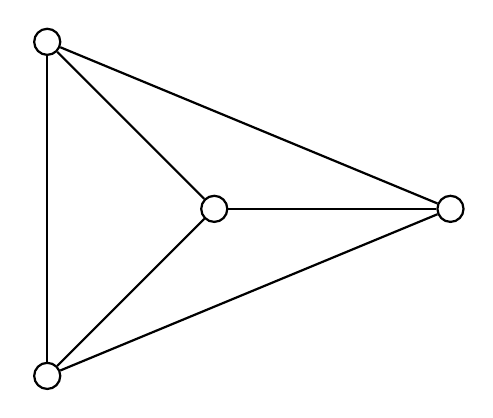
\begin{tikzpicture}[auto, node distance=3cm, every loop/.style={},
			thick,main node/.style={circle,draw,font=\sffamily\Large\bfseries}]
			
			\node[main node] (1) {};
			\node[main node] (2) [above left of=1] {};
			\node[main node] (3) [below left of=1] {};
			\node[main node] (4) [right of=1] {};
			
			\path[every node/.style={font=\sffamily\small}]
			(1) edge node {} (4)
			edge node {} (3)
			(2) edge node {} (1)
			edge node {} (4)
			(3) edge node {} (2)
			(4) edge node {} (3);
			\end{tikzpicture}
		}
	\end{center}
	
	
	Now let $G$ be a minimal nonplanar graph that is not a complete graph. By lemma \ref{component} $G$ contains connected component, $G'$, that is nonplanar. We know $G'\subset G$ and that all proper subsets of $G$ are planar, therefore $G'=G$. This means that $G'$ is the only component in $G$ so $G$ must be at least 1 connected.
	
	If $G$ is 1 connected then there exists some vertex $v$ for which $G\setminus\set v$ into at least two components. Let $H$ be one such component and $H'$ be the graph produced by adding $v$ back into $H$ ($H'$ is $v$ with all of $H$ and all edges between $H$ and $v$). Now $H'$ is a proper subgraph of $G$ so it must be planar. We also know that $G\setminus H$ is a proper subgraph of $G$ and therefore must also be planar. By lemma $\ref{outside}$ we may draw both $G\setminus H$ and $H'$ such that $v$ borders the outer face. We may split $\mathbb R^2$ into two disjoint subsets
	\begin{align*}
	R^- &= \setbuilder{\pair xy\in\mathbb R^2}{x < 0}\\
	R^+&=\setbuilder{\pair xy\in\mathbb R^2}{x > 0}
	\end{align*}	
	then draw $H'$ in $R^-$ with the exception of putting $v$ at $\pair 00$ and then draw $G\setminus H$ in $R^+$ with the exception of putting $v$ at $\pair 00$. This then yields a plane drawing of $G$, so $G$ must be at least 2 connected.
\end{proof}

\begin{definition}[lobe]
	Let $G$ be a graph with cut set $S$. Further let $C_1, C_2, \ldots C_n$ be the connected components of $G\setminus S$. A lobe $L_i$ of $S$ is then what we would get if we took the subset of $G$ containing all of $C_i$ and $S$. This can more formally be written as
	$$
	L_i = G\setminus \left(\unionacross{j\not=i}{C_j}\right)
	$$
\end{definition}

\begin{lemma}\label{lobes}
	Let $G$ be a nonplanar 2 connected graph with minimal cut set $S=\set{x,y}$. Further if $L$ is a lobe of $S$ let $L^+$ be the graph of $L$ with an edge added between $x$ and $y$. There exists some lobe $L$ of $S$ for which $L^+$ is nonplanar. 
\end{lemma}
%TODO cite http://www.cs.rpi.edu/~goldberg/14-GT/19-kurat.pdf
\begin{proof}
	Let $G$ be a graph with lobes $L_1, L_2, \ldots, L_n$ of separating set $S=\set{x,y}$. Suppose that for all $i$, $L_i^+$ is planar. We may then draw $L_1^+$ on the plane. If we have a planar drawing of $\unionfrom{j = 1}{i-1}{L_j^+}$ we can then embed a drawing of $L_i^+$ where the edge between $x$ and $y$ borders the outer edge into a face that is bordered by the edge between $x$ and $y$ in our planar drawing of $\unionfrom{j = 1}{i-1}{L_j^+}$. We then can redraw this embedding such that $x$ and $y$ in $L_i^+$ are at the same points as $x$ and $y$ in $\unionfrom{j = 1}{i-1}{L_j^+}$ yielding a planar drawing of $\unionfrom{j=1}{i}{L_j^+}$. By induction then $\unionfrom{i=1}{n}{L_i^+}$ is planar. Clearly $G \subset \unionfrom{i=1}{n}{L_i^+}$ so by lemma \ref{subgraph} we know $G$ must be planar.
\end{proof}

\begin{lemma}\label{3connect}
	If $G$ is a graph with the properties listed below, then $G$ is at least 3-connected.
	\begin{enumerate}
		\item $G$ does not contain any subgraph that is contactable to of $K_{3,3}$ or $K_5$.
		\item $G$ is nonplanar.
		\item Of all graphs satisfying properties (1) and (2), $G$ has the least number of edges.
		\item Of all graphs satisfying properties (1), (2) and (3), $G$ has the least number of vertices.
	\end{enumerate}
\end{lemma}
%TODO cite http://www.cs.rpi.edu/~goldberg/14-GT/19-kurat.pdf

\begin{proof}
	Let $G$ be a graph fitting the above properties. Any proper subgraph, $H$, of $G$ will be missing at least one vertex or one edge from $G$. If $H$ is missing a vertex from $G$, then $H$ must break one of the first 3 properties. $H$ can not contain a subgraph that is contactable to $K_{3,3}$ or $K_5$ as then $G$ would also contain it and $H$ can not have more vertices than $G$. This leaves only that $H$ must be planar. If $H$ is missing an edge from $G$, then $H$ must break one of the first 2 properties. Again $H$ can not contain a subgraph that is contactable to $K_{3,3}$ or $k_5$ as then $G$ would also contain it. This again leaves only that $H$ must be planar. This means that all proper subgraphs $H$ of $G$ are planar so $G$ is minimally nonplanar. Additionally we know that $G$ is not a complete graph as all complete graphs either contain $K_5$ or are planar.
	
	By lemma \ref{2connect} we know that $G$ is at least 2 connected. Suppose that $G$ is 2 connected. Let $\set xy = S$ be a cut set in $G$. We know by lemma \ref{lobes} that there is a lobe $L$ for which adding an edge between $x$ and $y$ would yield a nonplanar graph $L^+$. Clearly $L^+$ has less edges then $G$, so $L^+$ must contain a subgraph that is contractible to $K_{3,3}$ or $K_{5}$. Consider another lobe $M$ of $S$. There must be a path, $p$, from $x$ to $y$ in $M$ as otherwise $G$ would not be either 0 or 1 connected. Clearly $L\union p$ is a subgraph of $G$ and $L\union p$ is contractible to $L^+$. By lemma \ref{contractibleCarryOn} we then know that $L\union p$ contains a subgraph that is contractible to $K_{3,3}$ or $K_5$. This gives us a contradiction so $G$ can not be 2-connected and therefore must be at least 3 connected.
\end{proof}

\subsection{Bridges}

Let $G$ be a connected graph with cycle $C$. Let $G'$ be the graph of $G$ when all edges of $C$ are removed. 
\begin{definition}[partial bridge]
	A partial bridge, $B$, of $C$ in $G$ is any connected subgraph of $G'$ that contains at lest one edge and for any two edges $a$ and $b$ in $B$, there is a walk in $B$ that contains both $a$ and $b$ and does not pass through any vertex of $C$ (it may begin or end on with a vertex of $C$, but no internal vertex may be in $C$). 
\end{definition}
\begin{definition}[bridge]
	A partial bridge, $B$, is a bridge of $C$ in $G$ if there does not exist a partial bridge $B'\not=B$ of $C$ in $G$ such that $B\subset B'$.
	
	Alternatively a bridge is a maximal partial bridge.
\end{definition}

Bridges are the final tool we use to prove Kuratowski's theorem. We will now build up some lemmas, that we will need and might help us to build up a conception of a bridge. For these let $G$ be a connected graph with cycle $C$ and let $G'$ be the subgraph. All bridges and partial bridges will be in reference to $C$.


\begin{lemma}\label{walktopartialbridge}
	Let $W$ be a walk in $G'$ that does not pass through $C$ (it may start and end in $C$) and has at least one edge. Then the graph, $H$, composed of the vertices and edges in $W$ is a partial bridge.
\end{lemma}
\begin{proof}
	First $H$ is a subgraph of $G'$ as $W$ is a walk in $G'$. Second $H$ contains at least one edge as $W$ contains at least one edge. Third $H$ is connected trivially. Finally $W$ is a walk containing all edges of $H$ and not passing through $C$, so $H$ must be a partial bridge.
\end{proof}

\begin{lemma}\label{partialbridgeunion}
	Let $A$ and $B$ be partial bridges sharing a vertex, $v\not\in C$, then $A\union B$ is a partial bridge.
\end{lemma}
\begin{proof}
	First $A\union B$ is trivially a subgraph of $G'$ and contains at least one edge as both $A$ and $B$ contain at least one edge. Additionally $A\union B$ is connected as for any pair of vertices $a,b \in A\union B$ we have the following possibilities:
	\begin{itemize}
		\item If both $a$ and $b$ are in $A$ or both $a$ and $b$ are in $B$, then there is a walk from $a$ to $b$ within $A$ or $B$ respectively as both $A$ and $B$ are connected.
		\item Otherwise one of the vertices is in $A$ and the other is in $B$. Without loss of generality let $a\in A$ and $b\in B$, then we can construct a walk from $a$ to $v$ within $A$ as both are in $A$ and a walk from $v$ to $b$ as within $B$ both are in $B$. We then combine these two walks and have a walk from $a$ to $b$ that stays within $A\union B$.
	\end{itemize}
	Therefore $A\union B$ is connected. Finally we can make a similar argument that for any edges in $a,b\in A\union B$ there is a walk within $A\union B$ that doesn't pass through $C$ that contains both $a$ and $b$.
	\begin{itemize}
		\item If both $a$ and $b$ are in $A$ or both $a$ and $b$ are in $B$ then there is such a walk as $A$ and $B$ are both partial bridges.
		\item If $a$ and $b$ are not both in $A$ or both in $B$ then without loss of generality we can let $a\in A$ and $b \in B$. First as $A$ and $B$ are both connected and contain at least one edge, then $v$ must have at least one edge in each $A$ and $B$. Now we know there exists a walk in $A$ containing both $a$ and an edge of $v$ and there is a walk in $B$ containing both $b$ and an edge of $v$, and both these walks do not pass through $C$. Any walk passing though an edge of $v$ must also contain $v$, so both these paths must contain $v$. Without loss of generality we will assume the walk in $A$ contains $v$ after $a$ and the walk in $B$ contains $b$ after $v$. We now construct a walk that starts as the first walk up until has passed through $a$ and continued on to $v$, then we start following the walk in $B$ as it does after $v$ until reaching $b$. This walk's internal vertices are composed only of internal vertices from the walk in $A$, the walk in $B$ and of $v$. All of these are known not to be in $C$.
	\end{itemize}
	Now we have shown that $A\union B$ is a partial bridge.
\end{proof}

\subsubsection{Some more useful definitions about bridges}
\begin{definition}[vertex of attachment]
	If $B$ is a bridge of cycle $C$, then any vertex in both $B$ and $C$ is a vertex of attachment
\end{definition}

\begin{definition}[degree]
	The degree of a bridge is the number of vertices of attachment it has.
\end{definition}

\begin{corallary}
	No two bridges of the same cycle will share any edges and may only share a vertex if the vertex is in the cycle. 
\end{corallary}
\begin{proof}
	Let $A$ and $B$ be bridges of $C$. If they share a vertex that is not in $C$, then by lemma \ref{partialbridgeunion} we know that $A\union B$ is a partial bridge, and it would contain both $A$ and $B$, so then $A = A\union B = B$. If $A$ and $B$ share an edge, $e$, then they must also share the vertices of $e$. If either one of $e$'s vertices are not in $C$ then we already know that $A=B$. If both of $e$'s vertices are in $C$ then $e$ is the only edge in both $A$ and $B$ as for any other edge $e'$ a walk that contains both $e$ and $e'$ must through one of $e$'s vertices to get between $e$ and $e'$. Additionally neither $A$ nor $B$ can contain any other vertices than $e$'s vertices as they are connected. Therefore $A=B$ again.
\end{proof}

%Let $G$ be a connected graph with cycle $C$. We can define an equivalence relation $\sim$ on the set of all edges and vertices not in $C$ as $a\sim b$ if there is a walk, $v_1e_1v_2e_2\ldots v_{k-1}e_{k-1}v_k$, with the following properties.
%\begin{itemize}
%	\item All vertices $v_i$ with $1 < i < k$ are not on $C$. ($v_1$ and $v_k$ may be on $C$ but this is not a requirement.)
%	\item All edges in the walk must not be in $C$.
%	\item Both $a$ and $b$ must be in the walk, they may be either an edge or vertex.
%\end{itemize}
%We should check that this is a equivalence relation.
%\begin{itemize}
%	\item (\textit{symmetry}) - trivial from how we construct $\sim$.
%	\item (\textit{reflexivity}) - For a vertex $v$ we can define a walk with just $v$ and therefore $v\sim v$ as this walk fits our requirements. For an edge $e$, $e$ must have two vertices it is attached two, $a$ and $b$. We then construct a walk $aeb$, and therefore $e\sim e$.
%	\item (\textit{transitivity)} - If $a\sim b$ and $c$ then there is a walk that goes through both $a$ and $b$ and a walk that goes through both $b$ and $c$. None of $a$, $b$, or $c$ are on $C$ as $\sim$ is not defined on $C$. Any walk $W$ we can reverse the direction of and it will still fit our rules above. This means that we can say there is a walk that goes through $a$ and then through $b$ as well as a walk that goes through $b$ and then through $c$. These walks will then take the the form $\alpha_1\alpha_2\ldots\alpha_{k}$ and $\beta_1\beta_2\ldots\beta_n$ with $a = \alpha_i$, $b = \alpha_j = \beta_m$, and $c = \beta_o$ for some $1\le i \le j \le k$ and $1\le m \le o \le n$. Now if $b$ is a vertex we can construct a walk as follows:
%	$$\alpha_1\ldots\alpha_{i-1}a\alpha_{i+1}\ldots\alpha_{j-1}b\beta_{m+1}\ldots\beta_{o-1}c\beta_{o+1}\ldots\beta_n$$
%	giving us a valid walk containing both $a$ and $c$. If $b$ is an edge then $\alpha_{i-1}$ is a vertex adjacent to $b$ and thus it must appear either before or after $b$ in any walk including $b$ as an edge. Additionally we know $\alpha{i-1}$ is not part of $C$ as it is in the interior of our walk containing $a$ and $b$. Therefore we can construct a walk just like we did last time that starts at $\alpha_1$ then goes through $a$ and then up to $\alpha_{i-1}$ at which point it switches to the equivalent vertex in the other walk be it $\beta{m-1}$ or $\beta{m+1}$ and simply follows that walk through $c$ until it reaches $b_n$. This walk will contain both $a$ and $b$ and therefore we know $a\sim b$ in all cases.
%\end{itemize}
%Now we may consider the partition created by $\sim$ on the set of all vertices and edges not in $C$. For any partition $P$ then we may construct $\bar P$ as $P$ with any vertices in $C$ that an edge $P$ connects to. This $\bar P$ is then what we call a bridge. Lets take a bit to get an intrinsic understanding of what a bridge is.
%
%Conceptually a bridge is a sort of bit of the graph

\begin{lemma}
	Every bridge $B$ of cycle $C$ contains at least one vertex in $C$.
\end{lemma}
\begin{proof}
	Let $B$ be a partial bridge that does not contain any vertex in $C$. We know $C$ and $B$ are contained within a larger graph $G$ that is connected, so there must be a walk from any vertex in $B$ to any vertex in $C$. Consider then a walk $W$ that starts at vertex $b\in B$ and ends at vertex $c\in C$. There must be some first vertex in $W$ that is in $C$, so let us call $W'$ the subwalk of $W$ from $b$ to that first vertex in $C$. Now we know that $W'$'s first vertex in $C$ is also its last vertex, so it does not pass through $C$. Therefore by lemma \ref{walktopartialbridge} the graph $H$ composed of $W'$'s vertices and edges is a partial bridge. We know also that $B\union H$ is a partial bridge by lemma \ref{partialbridgeunion}. Finally $B\not=B\union H$ as $B\union H$ contains a vertex in $C$ and $B$ does not. Now we have a partial bridge, $B\union H$ that contains $B$, so we know $B$ is not a bridge.
\end{proof}

\begin{lemma}
	In a plane drawing of a graph $G$, given some cycle $C$, every bridge, $B$, of $C$ will either entirely be in the interior or exterior of $C$ with the exception of the vertices of $B$ that are in $C$.
\end{lemma}
\begin{proof}
	We know that $C$ splits the plane into the interior and exterior. We know every vertex and edge that are not in $C$, must be entirely in the interior or exterior. As $B$ is a subgraph $G'$ which contains no edges of $C$ then every edge in $B$ is entirely in the interior or exterior.
	
	Now assume for the sake of contradiction there is an edge, $e\in B$ that is in the exterior and an edge $i\in B$ that is in the interior. Then any walk containing both $e$ and $i$ must pass over $C$ which can only be done at vertices of $C$. This then means that every walk contain $e$ and $i$ passes through $C$ and thus we have a contradiction.
	
	Now for any vertex $v\in B$ there is some edge $e\in B$ that connects to $v$. If $v$ is in the interior of $C$ then $e$ must also be entirely in the interior, and if $v$ is in the exterior then $e$ must be entirely in the exterior. This means that if any part of $B$ is in the interior, then $B$ must have at least one edge in the interior and if any part of $B$ is in the exterior then $B$ must have at least one edge in the exterior. We then can conclude that all of $B$ must be solely in the interior of $C$ or the exterior of $C$.
\end{proof}



\subsection{The home stretch}
We can finally provide the proof for Kuratowski's theorem.

\THEBIGONE*

\begin{proof}
	Suppose that $G$ is a graph with the following properties.
	\begin{enumerate}
		\item $G$ does not contain any subgraph that is contactable to of $K_{3,3}$ or $K_5$.
		\item $G$ is nonplanar.
		\item Of all graphs satisfying properties (1) and (2), $G$ has the least number of edges.
		\item Of all graphs satisfying properties (1), (2) and (3), $G$ has the least number of vertices.
	\end{enumerate}
	We will try and show that $G$ does not exist.

	First off we have lemma \ref{3connect} which says that $G$ must be at least 3 connected. Additionally we know that $G$ must be minimally nonplanar.\footnote{This was proved in the beginning of the proof for lemma \ref{3connect}.} Now choose an edge $e \in G$ between $x$ and $y$ and let $G' = G\setminus\set e$. Clearly $G'$ is planar. Because $G$ is 3 connected, by Menger's theorem (theorem \ref{menger}) we know that between any two vertices $a\not=b$ there are at least 3 internally disjoint paths in $G$. From this we can see that in $G'$ there must be at least 2 internally disjoint paths between $a$ and $b$. This means that every pair of paths in $G'$ lie upon a cycle, start at $a$ go down one path to $b$, then follow the other internally distinct path back to $a$. Let $\mathcal C$ be the set of all cycles that $x$ and $y$ lie on in $G'$. Let $\mathcal D$ be the set of all plane drawings of $G'$. By lemma \ref{JordansLemma} we know that every drawing $D\in\mathcal D$ we know that all cycles $C\in\mathcal C$ form a Jordan curve. Now choose a pair $\pair CD \in \mathcal C\cross\mathcal D$ such the curve created by $C$ in $D$ has the maximum possible number of edges in its interior. Now lets take a look at the bridges of $C$ in $D$.
	
	$C$ has no bridges of degree 1 as their vertex of attachment would be a single vertex cut set and we know $G'$ is at least 2 connected. Now we can break $C$ into two parts. If we start at $x$ and travel along $C$ to $y$ we get a path we are calling $p$. If we continue along $C$ from $y$ back to $x$ we get another path $q$.
	
	Claim: There are no external bridges of $C$ that have more than one vertex of attachment in either $p$ or $q$.
	
	Proof: Assume there is an external bridge $B$ of $C$ with vertices of attachment $b_1$, $b_2$ with either both in $p$ or both in $q$. Let $r$ be the path (either $p$ or $q$) that contains $b_1$ and $b_2$. Further assume without loss of generality that $b_1$ comes before $b_2$ in $r$. As $B$ is connected, there must be a path $s$ in $B$ from $b_1$ to $b_2$. Now construct a path $r'$ that starts where $r$ starts, goes down $r$ to $b_1$ then follows $s$ to $b_2$ where it continues down $r$ until $r$'s end. If $b_2 = r_j$ this would look like
	$$
	r' = r_1r_2\ldots b_1s_1s_2\ldots b_2r_{j+1}r_{j+2}\ldots r_{\card r}
	$$
	Now we can construct $C'$ to be $C$ but replace $r$ with $r'$. $C'$ clearly contains both $x$ and $y$, and it also will have more edges on it's interior than $C$ did. This is a contradiction as $C$ is the cycle containing $x$ and $y$ with the most edges on the interior.
	
	Now by the pigeonhole principle there can not be any external bridges of $C$ with degree greater than 2. Further no external bridge may have $x$ or $y$ as a vertex of attachment as $x$ and $y$ are in both $p$ and $q$. This means that all external bridges of $C$ are degree two with one vertex of attachment in $p$ and one vertex of attachment in $q$ and neither in $\set{x,y}$. We also know there is at least one external bridge of $C$ as otherwise $x$ and $y$ would both be bordering the outer face so the edge $e$ can be drawn within the outer face yielding $G$ to be a planar graph. By similar logic there must be some internal bridge $I$ that has one vertex of attachment in $p\setminus\set{x,y}$ and one vertex of attachment in $q\setminus\set{x,y}$ (This is because if there was no such bridge $x$ and $y$ would share a face and we could draw in $e$ making $G$ planar).
\end{proof}

\end{document}